\documentclass{beamer}

\usepackage[utf8]{inputenc}
\usepackage{default}
\usepackage{graphicx}


\title[Kurzform]{A Particle State Visualisation Tool} 
\subtitle[Kurzform]{Arranging Quarks} 
\author[Kurzform]{Robert Czechowski, Fabian Wilk} 
\institute[Kurzform]{CERN} 
\date[Kurzform]{04. 08. 2013} 
%\titlegraphic{\includegraphics[width=0.4\textwidth]{../unigoelogo.pdf}}

\begin{document}

\frame{\titlepage}

\frame{
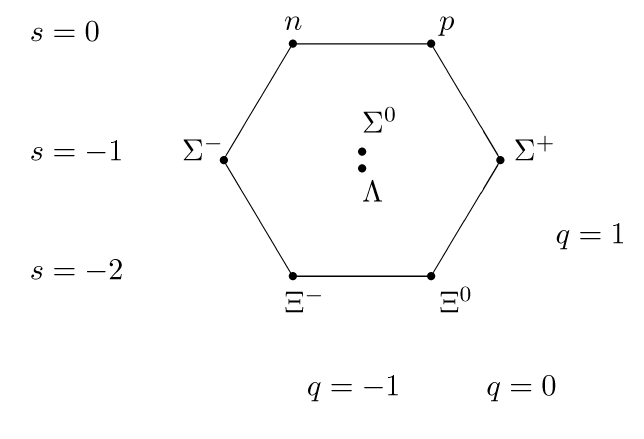
\includegraphics[width=.4\textwidth]{Baryon_octet.png}
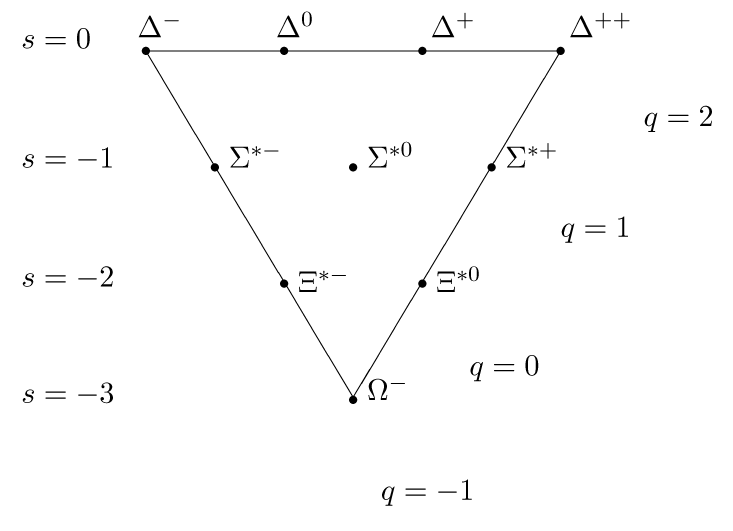
\includegraphics[width=.4\textwidth]{Baryon_decuplet.png}

From [Wikipedia].

Why are some combinations not possible in the octed?
}

\frame{
\begin{itemize}
 \item Has to do with spin and symmetry of states.
\item What would be cool: A visualisation of states to see how they look like, and how they transform according to various symmetry operators.
\end{itemize}
}
\frame{
We did this.
}

\frame{
\begin{itemize}
 \item Written in C++ (CGI) / HTML (+CSS). 
\item Supports Ket-Notation.
\item Due to lack of time:
\begin{itemize}
 \item Vadility checks only present in backend.
\item Additional symmetries only present in backend.
\item No general informations beeing displayed in box yet.
\end{itemize}
\end{itemize}
}

\frame{
We are:
\begin{itemize}
\item Rebecca Carney
\item Robert Czechowski
\item Nils Rosien
\item Fabian Wilk
\end{itemize}

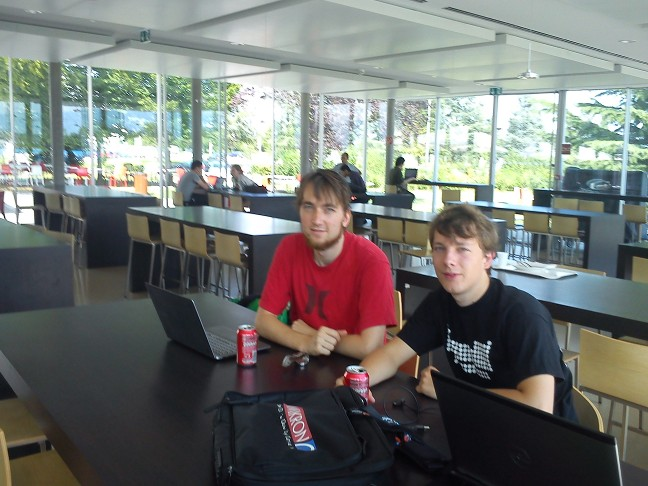
\includegraphics[width=.4\textwidth]{../graphics/foto.jpg}
}


\frame{
Thank you for your attention.
}

\end{document}
